\section{Study 2: CIFAR-10 Ablation}
\label{sec:study2}

\subsection{Training Outcomes}

Table~\ref{tab:outcomes} presents the central result: only 1 of 8 cells converged.

\begin{table}[H]
\centering
\caption{Training outcomes for all 8 cells. Best FID is the minimum across 15 solver/NFE combinations.}
\label{tab:outcomes}
\small
\begin{tabular}{@{}cccccrr@{}}
\toprule
Cell & Coupling & Objective & Estimator & Status & Best FID & Ckpt \\
\midrule
000 & Indep. & CFM & Uniform & \textcolor{red}{NaN} & 679.2 & 10k \\
001 & Indep. & CFM & TPC & \textcolor{red}{NaN} & 419.8 & 10k \\
010 & Indep. & StableVM & Uniform & \textcolor{orange}{Unstable} & 256.8 & final \\
011 & Indep. & StableVM & TPC & \textcolor{orange}{Unstable} & 197.9 & final \\
\textbf{100} & \textbf{BatchOT} & \textbf{CFM} & \textbf{Uniform} & \textcolor{green!60!black}{\textbf{OK}} & \textbf{18.4} & \textbf{final} \\
101 & BatchOT & CFM & TPC & \textcolor{red}{NaN} & 679.2 & 10k \\
110 & BatchOT & StableVM & Uniform & \textcolor{orange}{Unstable} & 211.4 & final \\
111 & BatchOT & StableVM & TPC & \textcolor{orange}{Unstable} & 273.6 & final \\
\bottomrule
\end{tabular}
\end{table}

Three patterns are immediate: (i)~BatchOT is necessary but not sufficient---cell\_100 converged, but 101/110/111 did not; (ii)~TPC causes NaN in every configuration (001, 101); (iii)~StableVM causes extreme loss oscillation (${\sim}40$ to ${\sim}22{,}000$) in all four cells where it appears (010, 011, 110, 111).

\subsection{Cell\_100: The Only Successful Model}

Figure~\ref{fig:cell100_fid} shows the FID--NFE trade-off for cell\_100. Training loss decreased smoothly from 0.54 to 0.14 over 80k steps. Midpoint is the most efficient solver, reaching FID~20.4 at NFE=40---matching Euler at NFE=100, a $2.5\times$ efficiency gain consistent with Study~1's trajectory-straightness findings. RK4 achieves the best absolute FID of 18.4 at NFE=100.

\begin{figure}[H]
    \centering
    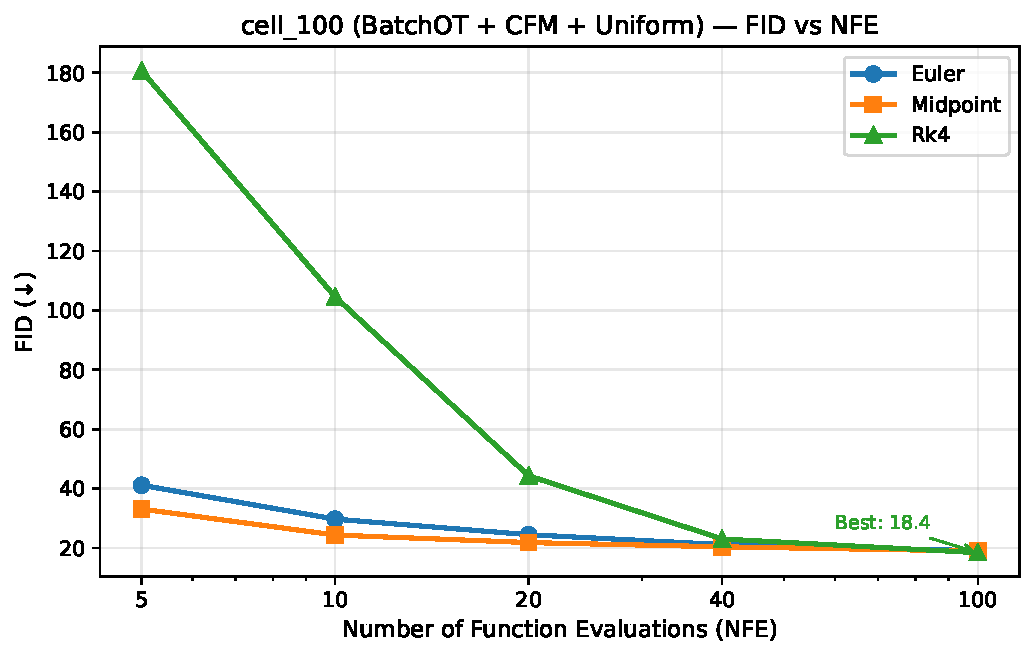
\includegraphics[width=0.65\textwidth]{figures/combined/cell_100_fid_detail.pdf}
    \caption{FID vs.\ NFE for cell\_100 (BatchOT + CFM + Uniform). Midpoint dominates at low NFE; RK4 wins at high NFE.}
    \label{fig:cell100_fid}
\end{figure}
